\input{template_files/packages}
\usepackage{units}
%\usepackage[T1]{fontenc}
%\usepackage[utf8]{inputenc}
\usepackage{physics}

\newcommand{\ee}{\mathrm{e}}
\newcommand{\ii}{\mathrm{i}}

\title{H1b: MD simulation -- dynamic properties}
\author{Andr\'eas Sundstr\"om and Linnea Hesslow}
\date{\today}

\begin{document}

\input{template_files/titlepage}

\section*{Introduction}

The velocity Verlet algorithm is a semi-implicit and efficient method to simulate an ensemble of particles whose trajectories are governed by Newton's equation of motion. Accordingly, it is a suitable algorithm to study molecular dynamics and to determine statistical properties of a system. Here, we use the velocity Verlet algorithm to study a system of aluminum atoms in a face centered cubic (FCC) lattice. By scaling the positions, momenta and lattice parameter, we can equilibrate the temperature and pressure to prescribed values. We  study the alumninum system at \unit[500]{$^\circ$C} and \unit[700]{$^\circ$C}, which correspond to the solid and liquid state respectively, and compute two dynamic quantities:   
mean squared displacements and the velocity correlation function.

For this report, we used scripts provided by Anders Lindman for intializing FCC lattices and calcualting lattice energies, lattice forces and virials of an aluminium lattice. All simulations were done in a simulation box containing $4^3=64$ unit FCC cells, and a total of $4\cdot64$ aluminum atoms placed at the corresponding FCC lattice points. The simulation box had periodic boundary conditions.

\subsubsection*{The velocity Verlet algorithm}
The main idea behind the velocity Verlet algorithm is to split up the time steps of the velocity, in order to make the update process of the state more symmetric. The position, velocity and acceleration, $x_i$, $v_i$ and $a_i$\footnotemark{} respectively, are updated according to
\footnotetext{In most situations the acceleration need not be saved for each time step, which might be insinuated by the index on $a_i$. The index is just used for notational convenience. }
\begin{equation}
\begin{aligned}
v_{i+\tfrac{1}{2}}=& v_{i}+\frac{1}{2}a_{i}dt,\\
x_{i+1} =& x_{i} + v_{i+\tfrac{1}{2}}dt,\\
a_{i+i} =& \mathtt{get\_acceleration}(x_{\i+1}),\\
v_{i+1} =& v_{i+\tfrac{1}{2}} + \frac{1}{2}a_{i+1}dt.\\
\end{aligned}
\end{equation}
By effectively using an average of the old and new acceleration, $(a_{i+1}+a_{i})/2$, for updating the velocity, $v_{i}\to v_{i+1}$, the velocity Verlet algorithm becomes semi-implicit; this also results in better energy-conservation properties of the algorithm, compared to, e.g., a fully explicit algorithm ($v_{i+1}=v_{i}+a_{i}dt$). However, in contrast to a fully implicit algorithm, there is no need for a computationally costly matrix inversion for each time step, and the velocity Verlet algorithm is also self-starting on an initial condition of $x_{i=0}=x_0$, $v_{i=0}=v_0$, and $a_{i=0}=\mathtt{get\_acceleration}(x_{0})$.



\section*{Task 1: potential energy}
The theoretical, minimum energy lattice parameter for aluminum can be determined by calculating the minimum potential energy per unit cell in a lattice with zero initial momenta for all particles. 

Figure~\ref{fig1} shows the potential energy as a function of the lattice parameter. We used a quadratic fit to find the minimum energy\footnote{We performed the quadratic fit in the volume $V$, which to a small error corresponds to a quadratic fit in the lattice parameter $a$, since $E \approx  \alpha(V-V_0)^2 \approx \alpha a_0^4 (a-a_0)^2$ in a close vicinity of the minimum $a\approx a_0$.}, and obtained $V_{\rm eq} \approx \unit[65.38]{\AA^3}$. This corresponds to the equilibrium lattice parameter $a_{\rm eq} \approx \unit[4.029]{\AA}$ at \unit[0]{K}, which we took as the initial lattice parameter for the following tasks.  We find that figure~\ref{fig1} looks similar to the figure~1 in the homework problem file, which is encouraging.
\begin{figure}[!ht]
\begin{center}
  \includegraphics[width=0.7\textwidth]{../figures/potential_energy} 
  \caption{The potential energy per unit cell for aluminum as a function of the lattice parameter cubed.}
  \label{fig1}
\end{center}
\end{figure}



%%%%%%%%%%%%%%%%%%%%%%%%%%%%%%%%%%%%%%%%%%%%%%%%%%%%%%%
\section*{Task 2: determine the time step}
In this task, we use a lattice with the equilibrium lattice constant $a_{\rm eq} \approx \unit[4.029]{\AA}$, found in the previous task, but then we added a random perturbation, uniformly distributed in the interval $\pm0.065a_{\rm eq}$, to each atom position. This creates a non-equlibrium system, which has a non-trivial time evolution. To determine the time evolution, we used the velocity Verlet algorithm, as described in the introduction.

The first step when doing simulations of this kind is to determine a suitable timestep. Even though the velocity Verlet algorithm have good energy conservation properties, it only gives an approximation to the ``true'' continuous solution; an approximation which gets better the smaller $dt$ we choose. However, choosing $dt$ too small will result in unnecessary computational costs for the same total simulation time. We are therefore interested in finding the largest $dt$ we can get away with without loosing energy conservation. From figure~\ref{fig:task2}, we see that $dt = \unit[2 \cdot 10^{-2}]{ps}$ clearly does not conserve energy, while $dt = \unit[1 \cdot 10^{-1}]{ps}$ dose conserve energy. To be on the safe side, we chose $dt = \unit[5 \cdot 10^{-3}]{ps} = \unit[5]{fs}$ as our time step. This is in line with the lecture notes, where it is stated that a suitable time step would normally be a few femtoseconds, or somewhat larger for heavy atoms.

The total energy of the simulated system at each time step is determined by sum of the kinetic energy of each particle, $E_{\rm kin}^{\rm(atom)}=\,m_{\rm Al}v^2/2$, and the total lattice energy of the system. Then, to calculate the temperature, we can use the \emph{equipartition theorem} stating that $\ev{E_{\rm kin}^{\rm(atom)}}=3k_{\rm B}T/2$, or equivalently that $T=2\ev{E_{\rm kin}^{\rm(atom)}}/(3k_{\rm B})$. We can therefore define an instantaneous temperature
\begin{equation}
\label{eq:T_instantaneous}
\mathcal{T}(t)=\sum_{\text{all atoms}}2E_{\rm kin}^{\rm(atom)}(t)/(3N_{\rm atoms}k_{\rm B}).
\end{equation}


\begin{figure}[!ht]
\begin{center}
  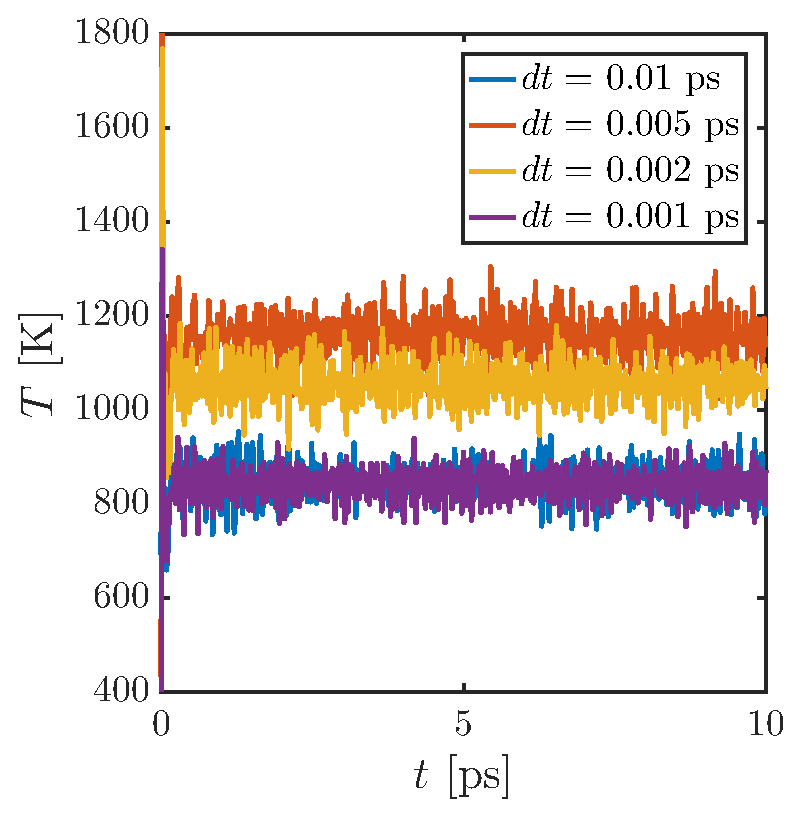
\includegraphics[width=0.48\textwidth]{../figures/dt-scan-temperature} 
    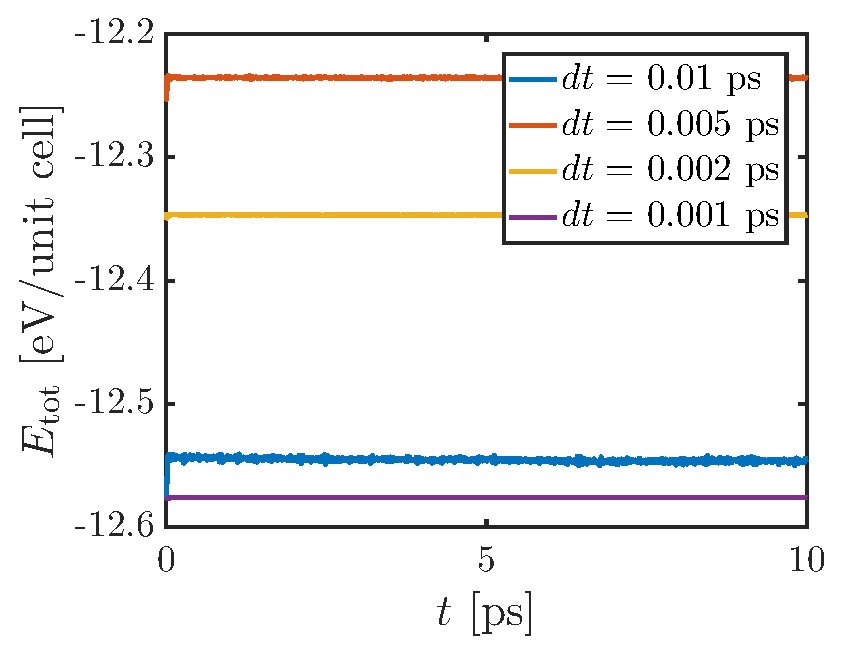
\includegraphics[width=0.48\textwidth]{../figures/dt-scan-energy} 
  \caption{The temperature and kinetic energy per unit cell as a function of time for four different time steps.}
  \label{fig:task2}
\end{center}
\end{figure}

With the random noise, the temperature and the energy differ between runs, but are in the same order of magnitude. 
We note that the temperature in several cases is higher than desired value of~\unit[600-800]{K} from the problem sheet. The temperatures and energies up to one standard deviation are quantified in table~\ref{tab:task2}.

\begin{table}[!ht]
  \begin{center}
    \caption{Energies and temperatures with one standard deviation uncertainties for four different values of the time steps.}
    \begin{tabular}{l c c} 
    $dt$ [ps] & $T$ [K] & $E_{\rm tot}$ [eV/unit cell]\\ \hline
$2 \cdot 10^{-2}$ & 	unstable &	unstable \\
$1\cdot 10^{-2}$ & 	$783 \pm 3.5\%$ &	$-12.61 \pm 9.2\cdot 10^{-3} \% $\\
$5\cdot 10^{-3}$ &	$793 \pm 3.7 \% $ &$-12.62 \pm 2.2\cdot 10^{-3} \%$ \\
$2\cdot 10^{-3}$ & $769  \pm 3.7 \% $ & 	$ -12.65 \pm 5.2\cdot 10^{-4} \% $\\ 
%$1\cdot 10^{-3}$ & $ 841  \pm 3.7 \% $	 &$ -12.58 \pm 3.6\cdot 10^{-4} \%$ \\ 
      \hline
    \end{tabular}
    \label{tab:task2}
  \end{center}
\end{table}


\section*{Tasks 3 and 4: temperature and pressure equilibration}
%When we started the system with the random fluctuations, we saw in figure~\ref{fig:task2} that we get some different temperatures each time. If we want to study the system at some given temperature and pressure, we need some way of persuading the system to change to the desired macro state.
There is no simple method to initialize a system to a specified temperature and pressure, but prescribed values can be obtained by scaling the velocities and the positions of the particles in the system. 
Given that the temperature of the system is given by the average kinetic energy of the atoms, we can change the temperature by scaling the velocities of all atoms. A scheme for this temperature scaling is to first calculate the instantaneous temperature $\mathcal{T}$ according to equation~\eqref{eq:T_instantaneous}, at that time step, and then scale it by a scaling factor
\begin{equation}
\alpha_T=1-\frac{dt}{\tau_T}\frac{\mathcal{T}-T_{\rm eq}}{\mathcal{T}},
\end{equation}
where $T_{\rm eq}$ is the desired equilibrium temperature, and $\tau_T$ turns out to be a typical time scale on which the system equlibrates. However, as we only have direct control of the particle velocities, we equilibrate the temperature by scaling the velocities by $v_i\to\sqrt{\alpha_T}v_i$, since the temperature depends quadratically on the velocities.

A similar scheme for pressure equlibration is to instead scale the particle positions and simulation-box volume, using a scaling factor of
\begin{equation}
\alpha_P=1-\kappa\frac{dt}{\tau_P}(\mathcal{P}-P_{\rm eq}),
\end{equation}
where $\mathcal{P}$ is the instantaneous pressure, $P_{\rm eq}$ is the desired equilibrium pressure, $\tau_P$ is the characteristic equlibration time, and $\kappa$ is the isothermal compressibility of the material simulated\footnotemark{}. This time the positions are scaled according to $x_i\to\alpha_P^{1/3}x_i$, and similarly the simulation box volume is scale by scaling its side lengths by $L\to\alpha_P^{1/3}L$.
\footnotetext{The isothermal compressibility is defined according to $\kappa=-(V\pdv*{P}{V})_T^{-1}$. This compressibility should therefore be used when scaling the volume of the box to change the pressure.}

We set $\tau_P = \tau_T = 100 dt$, where $dt = 5\cdot 10^{-3}$\,ps, and equilibrated the temperature and pressure by scaling the particle momenta and positions (and box size) respectively. Choosing a slower equilibration time did not affect the results qualitatively. Both temperature and pressure were equilibrated in the same Verlet loop, but for the higher temperature the system was first melted by increasing the temperature to \unit[1100]{$^\circ$C}. To determine the isothermal compressibility $\kappa$, 
the values of Young's modulus $Y$ and shear modulus $G$ were taken from Physics Handbook, table T 1.1. From F 1.15 in Physics Handbook, the bulk modulus can then calculated as
\begin{equation}
B = \frac{YG}{9G - 3Y} \,\quad \kappa_{\rm Al} = \frac{1}{B} \approx
\qty(\unit[6.6444\cdot 10^5]{bar})^{-1},
\end{equation}
where \unit[1]{bar } = $\unit[6.2415\cdot 10^{-7}]{eV/\AA^3}$ in atomic units.
%However, we set $\kappa = \kappa_{\rm Al}$ since the pressure equilibration happened on a much longer timescale than $\tau_P$ with $\kappa = \kappa_{\rm Al}$. We have not yet figured out why this is. 

The results are shown in figure~\ref{fig:eq}, where we overlay the instantaneous values of $\mathcal{T}$ and $\mathcal{P}$ with a moving average using 100 time steps. The desired temperatures and pressures were approximately obtained in the equilibration process. The averages during the last half of the process ($t \geq 10 \tau_{\rm eq}$), were
\begin{equation}
T=\unit[500\pm 29]{^\circ C},\quad  P = \unit[43 \pm 1232]{bar},
\label{eq:Tprod1}
\end{equation} 
and 
\begin{equation}
T=\unit[701\pm 34]{^\circ C},\quad P = \unit[-349 \pm 1911]{bar}.
\label{eq:Tprod2}
\end{equation}
The fluctuations in the pressure may appear large, but are roughly consistent with the fluctuations in the temperature (as well as figure~2 in the homework problem document). With $P = N k_{\rm B} T + W$, the fluctuations in the pressure can be estimated by
\begin{equation}
\Delta P = \sqrt{\Delta P_{\rm T}^2 + \Delta P_{\rm W}^2}, 
\end{equation} 
where
\begin{align}
\Delta P_{\rm T} &\equiv \frac{N k_{\rm B}}{V} \Delta T = \frac{4 k_{\rm B}}{a_0^3} \Delta T \approx 
\begin{cases}
\unit[234]{bar} \approx  \unit[0.02]{GPa}, \quad T=\unit[500]{^\circ C} \\
\unit[259]{bar} \approx  \unit[0.03]{GPa}, \quad T=\unit[700]{^\circ C}
\end{cases} \\
 \Delta P_{\rm W} &\equiv \frac{\Delta W}{V}.
\end{align}
The fluctuations $\Delta P$ in equations~\eqref{eq:Tprod1} and~\eqref{eq:Tprod2} are significantly larger than $\Delta P_{\rm T}$, but differ with less than an order of magnitude. We find it plausible that $\Delta P_{\rm W}$ can be significantly larger than $\Delta P_{\rm T}$. 


\begin{figure}[!ht]
\begin{center}
  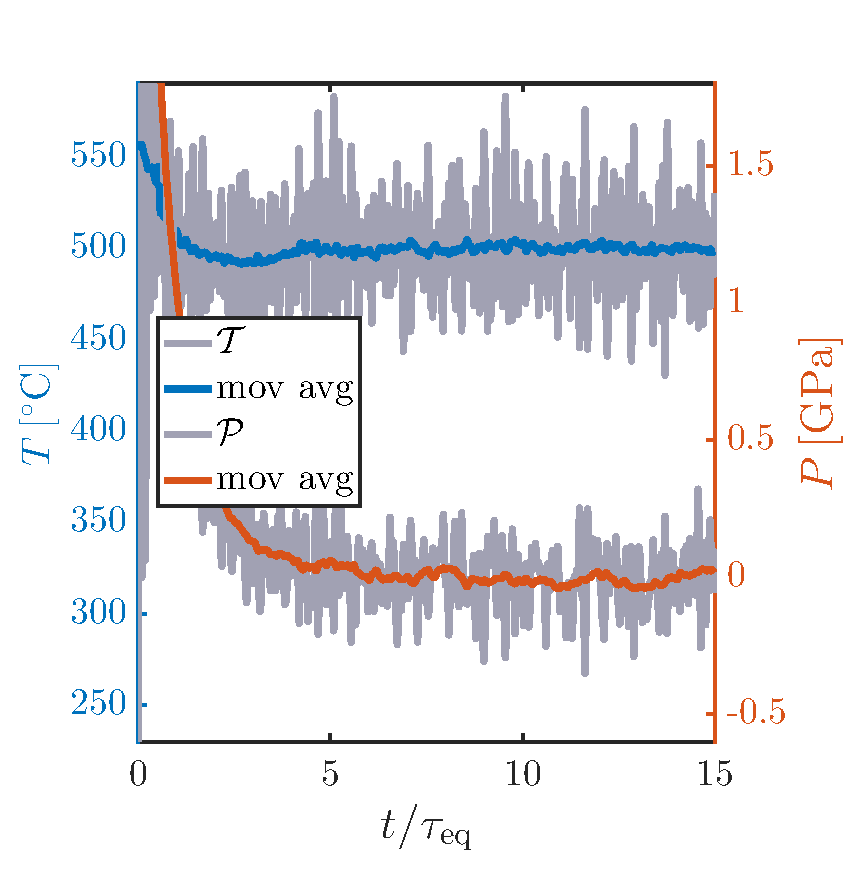
\includegraphics[width=0.48\textwidth]{../figures/TP-eq-500} 
    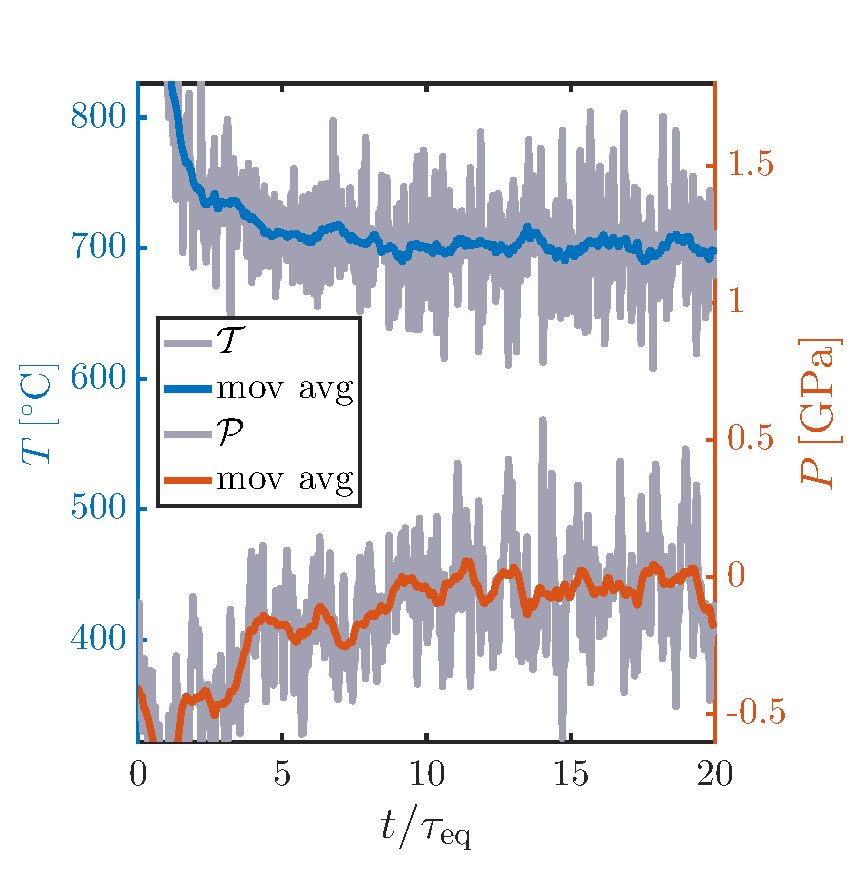
\includegraphics[width=0.48\textwidth]{../figures/TP-eq-700} 
  \caption{The instantaneous values of $\mathcal{T}$ and $\mathcal{P}$ overlaid with with a moving average using 100 time steps, which corresponds to $\Delta t = \tau_P/2$. Left panel: $T=\unit[500]{^\circ C}$,  right panel: $T=\unit[700]{^\circ C}$.}
  \label{fig:eq}
\end{center}
\end{figure}

Due to the large fluctuations, it is difficult to determine if the system has reached its equilibrium directly from the instantaneous pressure. Instead, we consider the time-evolution of the lattice parameter $a_0$, as shown in figure~\ref{fig:a0}. After $t = 20 \tau_{\rm eq}$, the lattice parameter has reached a constant which means that the equilibrium is reached. The equilibrium values of the lattice parameter were found to be 
\begin{align}
a_0 &\approx \unit[4.09]{\AA}, \quad T=\unit[500]{^\circ C}, \\
a_0 &\approx \unit[4.25]{\AA}, \quad T=\unit[700]{^\circ C} .
\end{align} 
These value are larger than the zero-temperature constants, and it is reasonable that the higher $\unit[700]{^\circ C}$ case corresponds to a larger lattice parameter at constant pressure. 
\begin{figure}[!ht]
\begin{center}
  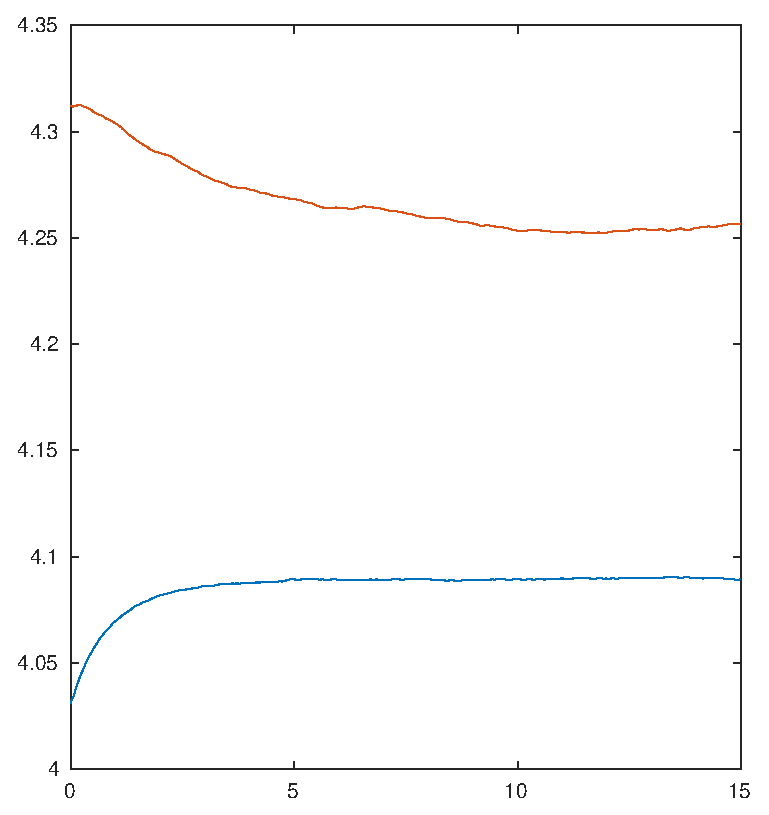
\includegraphics[width=0.7\textwidth]{../figures/a0}  
  \caption{The time evolution of the lattice parameter $a_0$ as the system equilibrates.}
  \label{fig:a0}
\end{center}
\end{figure}



\section*{Tasks 3-5: particle trajectories}
Starting with the temperature- and pressure-equilibrated systems from the previous section, we study the particle trajectories for both systems. Here, we decrease the time step to   $dt       = \unit[1\cdot 10^{-3}]{ps}$ and the simulation length to $t_{\rm end} = \unit[10]{ps}$ to get better statistics. This was mostly motivated by increasing the resolution in tasks 6-7. 

First, we note that the cumulative averages of the instantaneous temperatures and pressures stayed close to their initial values. This is shown in figure~\ref{fig:prod}. Numerically, we obtained 
\begin{equation}
T=\unit[504\pm 29]{^\circ C},\quad  P = \unit[-660 \pm 1215]{bar},
\label{eq:Tprod11}
\end{equation} 
and 
\begin{equation}
T=\unit[706\pm 37]{^\circ C},\quad P = \unit[-1021 \pm 1985]{bar}.
\label{eq:Tprod22}
\end{equation} 

\begin{figure}[!ht]
\begin{center}
  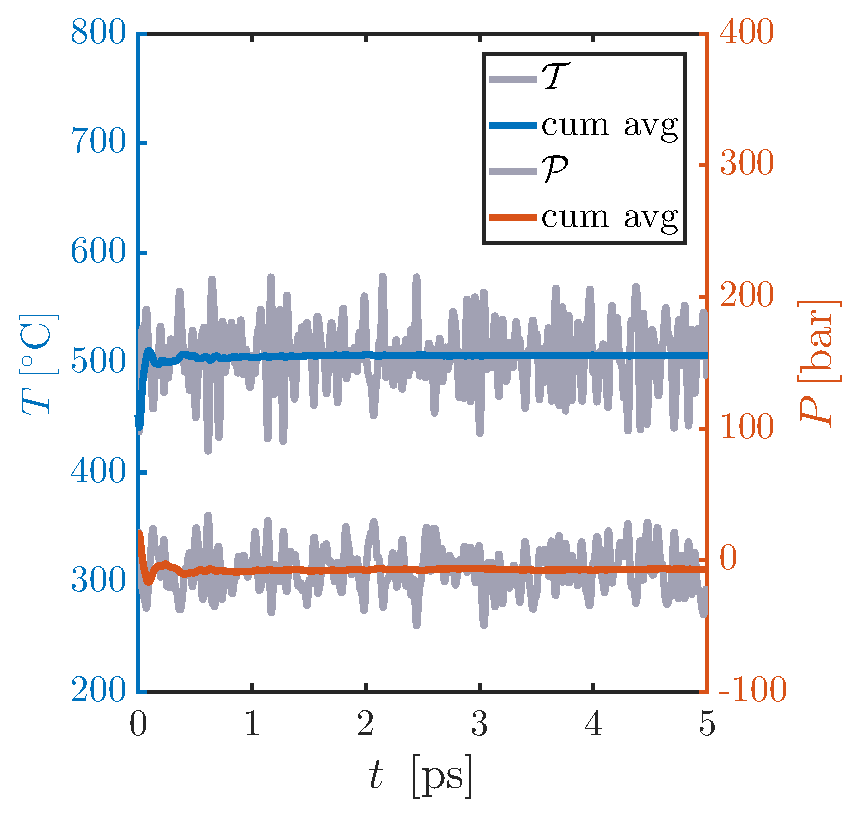
\includegraphics[width=0.48\textwidth]{../figures/TP-prod-500} 
    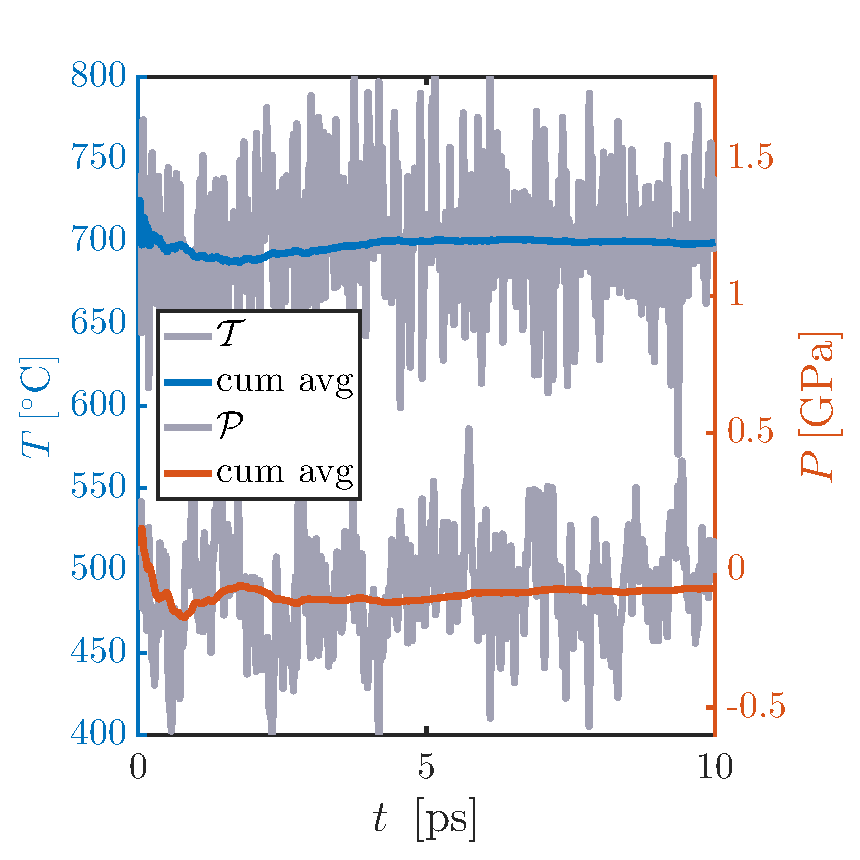
\includegraphics[width=0.48\textwidth]{../figures/TP-prod-700} 
  \caption{The instantaneous values, and the cumulative averages, of the temperature and the pressure in the production runs. Left panel: $T=\unit[500]{^\circ C}$,  right panel: $T=\unit[700]{^\circ C}$}
  \label{fig:prod}
\end{center}
\end{figure}

From equation (82) in MD lecture notes, the mean squared displacement can be calculated as
\begin{align}
\Delta_{\rm MSD}(t) &= \lim_{T \rightarrow \infty} \frac{1}{T} \int_0^{T} d t' \frac{1}{N_{\rm atoms}} \sum_{i=0}^{N_{\rm atoms}-1} \left[{\bf r}_i(t+t') - {\bf r}_i(t') \right]^2 \\ &\Rightarrow \nonumber
\\
\Delta_{\rm MSD}(t_k) &\approx
\frac{1}{N -k}\frac{1}{N_{\rm atoms}} \sum_{j=0}^{N-k-1} \sum_{i=0}^{N_{\rm atoms}-1} \left[{\bf r}_i(t_{k+j}) - {\bf r}_i(t_j) \right]^2 .
\label{eq:1}
\end{align}
Note that the sum over $j$ has a varying number of terms depending on $k$. For high $k$ (large $t_k$), the sum contains fewer terms and thus the statistics going into the average becomes less certain. The standard deviation in the mean is proportional to $(N-k-1)^{-1/2}$; hence when $k$ is large, the uncertainty also becomes large. However, note that \eqref{eq:1} utilizes the maximum amount of data, and the higher uncertainty at large $t_k$ cannot be avoided.


\begin{figure}[!ht]
\begin{center}
  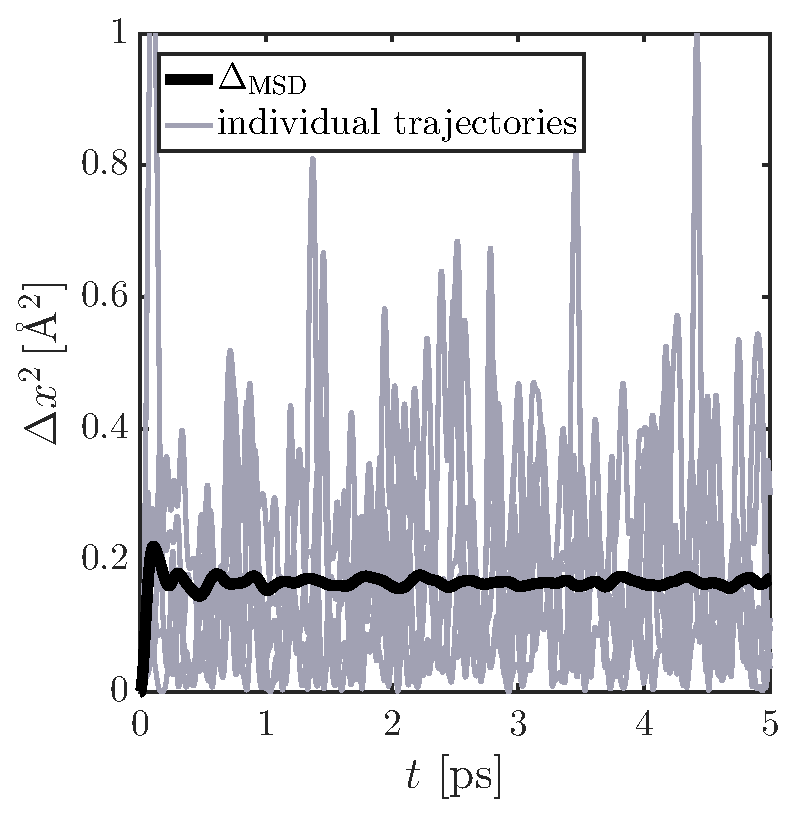
\includegraphics[width=0.7\textwidth]{../figures/MSD-500}  \\
    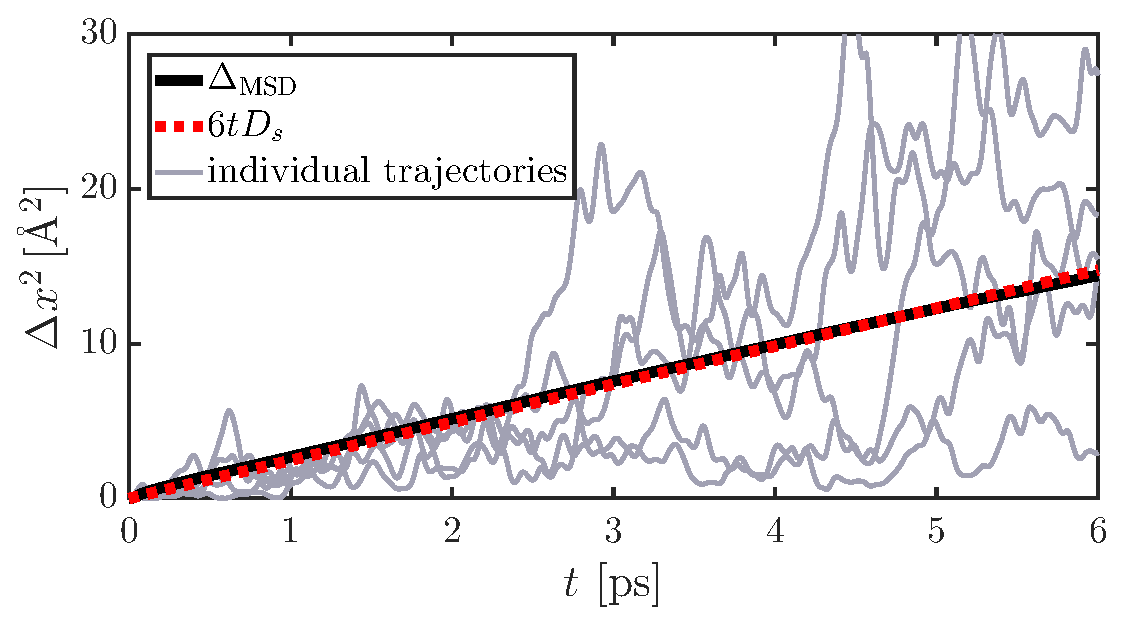
\includegraphics[width=0.7\textwidth]{../figures/MSD-700} 
  \caption{Five individual particle trajectories (gray thin lines), overlaid with the mean squared displacement $\Delta_{\rm MSD} \approx \unit[0.16]{\AA^2}$ (thick black line). In the top panel, $T=\unit[500]{^\circ C}$, the system is in a solid state. In the bottom panel, $T=\unit[700]{^\circ C}$, the system is in a liquid state, where $\Delta_{\rm MSD} \approx 6 t D_s$ (dotted red line).}
  \label{fig:MSD}
\end{center}
\end{figure}
We now consider the particle trajectories. Figure~\ref{fig:MSD} shows the trajectories of five individual particles along with the mean squared displacement as determined in equation~\eqref{eq:1}. We can clearly see that the particle trajectories are bounded in the left figure~\ref{fig:MSD}, while for the high-temperature case in the right panel, they increase as square root of time ($\Delta_{\rm MSD} \propto t$). Consequently, the former is in a solid state while the latter is in a liquid state.  
In the solid, the obtained mean squared displacement was $\Delta_{\rm MSD} \approx \unit[0.16]{\AA^2}$.

We determined the self-diffusion coefficient as the average slope of the mean squared displacement for $\unit[1]{ps} \leq t \leq \unit[9]{ps}$, yielding $D_s \approx \unit[0.42]{\AA^2/ps}$. This is because we want to avoid giving too much statistical significance to the values of $\Delta_{\rm MSD}(t)$ at high $t$, where the statistics are poor. 
In contrast, the method suggested, $D_s=\lim_{t\to\infty}\Delta_{\rm MSD}(t)/(6t)$, only utilizes the high uncertainty values of $\Delta_{\rm MSD}(t)$ at high $t$.



\section*{Tasks 6-7: velocity correlation and power spectrum}

We calculate the discrete auto-correlation function similarly to the MSD, in \eqref{eq:1}, 
\begin{equation}
\varPhi_k = \frac{1}{N-k}\sum_{i=0}^{N-k-1} \ev{v_{i+k}v_{i}}, \label{eq:Phi}
\end{equation}
where $j=0,1,\ldots,N-1$ and the average is taken over all atoms. Figure~\ref{fig:spectrum}(left) shows that it is noticeably different between the solid and the liquid states: while the solid state remains non-zero at longer time, presumably because of oscillations around lattice points, the liquid velocity correlation quickly decays to zero after some initial oscillations. Note that this calculation of $\varPhi_k$ suffers from the same high uncertainty at large $k$ as the MSD calculation.

\begin{figure}[!ht]
\begin{center}
  \includegraphics[width=0.7\textwidth]{../figures/Phi-t} \\
    \includegraphics[width=0.7\textwidth]{../figures/P-freq} 
  \caption{Top panel: The velocity correlation function, and (bottom panel) its spectrum, calculated both directly from the velocity correlation (solid line) and from the power spectrum of the particle velocity (dotted line). Blue lines show $T=\unit[500]{^\circ C}$ and red lines $T=\unit[700]{^\circ C}$.   
  %The spectrum is multiplied by a factor of $\tfrac{1}{2} m_{\rm Al}$, in which case it can be interpreted as energy per frequency interval and atom. 
  }
  \label{fig:spectrum}
\end{center}
\end{figure}


We now proceed to numerically approximate the integral
\begin{equation}
\hat{\varPhi}(f) = 2\int_0^{\infty}\dd{t}\,
\varPhi(t) \cos(2\pi ft)
\approx 2\int_0^{T_{\rm s}}\dd{t}\,\varPhi(t) \cos(2\pi ft)
\end{equation}
using a trapezoidal method in \textsc{Matlab}, with a frequency range $f=0$ to $f=1/(2\Delta{t})=f_{\rm Nyqvist}$, and frequency steps $\Delta{f}=1/T_{\rm s}$, where $T_{\rm s} = 0.75T$.
This is to avoid including noisy data in $\varPhi(t)$ at long time intervals $t$, where the statistics are poor---c.f. the discussion on the error in \eqref{eq:1}. Since that statistical ``noise'' will affect all frequencies, the solid lines in the lower panel of figure~\ref{fig:spectrum} would otherwise be too noisy.

We may then calculate the power spectrum according to
\begin{equation}
\begin{aligned}
\hat{P}(\omega) =& \lim_{T\to\infty}\frac{1}{T}
\ev{\abs{\int_0^{T}\dd{t}\,v(t)\ee^{\ii\omega t}}^2}\\
\approx& \frac{1}{T}
\ev{\abs{\int_0^{T}\dd{t}\,v(t)\ee^{\ii\omega t}}^2}\\
\Rightarrow\quad
\hat{P}_k=& \frac{1}{T}
\ev{\abs{\frac{T}{N} \sum_{i=0}^{N-1} v_i\exp(\ii2\pi\frac{ik}{N})}^2}
=\frac{T}{N} \ev{\abs{\hat{\vb*v}_k}^2}
\end{aligned}
\label{eq:PHat}
\end{equation}
where the averages is taken over all atoms, and
\begin{equation}
\hat{\vb*v}_k = \sqrt{N}\sum_{i=0}^{N-1} \vb*v_i \exp(\ii2\pi\frac{ik}{N})
\end{equation}
is the discrete Fourier transform of $v_i$. Note that the factor of $T$ was not included in the C scripts, and we therefore multiplied by this factor in the \textsc{Matlab} plotting scripts. When we compare $\hat{\varPhi}_k$ and $\hat{P}_k$ in figure~\ref{fig:spectrum} (right), we find that they are very similar, as, indeed, they should be according to the Wiener-Khinthchine theorem. If we instead take $T_s = T$ (using the full time evolution of $\Phi(t)$, we get a more noisy signal. This is because there is less statistics at high values of $j$ in equation~\eqref{eq:Phi}.
Therefore, even though the results are similar, the power spectrum method in equation~\eqref{eq:PHat} should be considered more accurate since it includes more statistics of the data points. 

The self-diffusion coefficient as determined by the power spectral density at $f=0$, was found to be  $D_{s, \hat \Phi} = \unit[0.38]{\AA^2/ps}$ and $D_{s, \hat P} = \unit[0.41]{\AA^2/ps}$ determined from $\hat \Phi$, and  $\hat P$ respectively. As expected, these values are close to the values obtained from the mean squared displacement. We note that $D_{s, \hat P}$ provides a better agreement with the $\Delta_{\rm MSD}$ value, which is consistent with $\hat P(\omega)$ containing more statistics.  

\section*{Concluding discussion}
Using the velocity Verlet algorithm, we study a system of aluminum atoms  at \unit[500]{$^\circ$ C} and \unit[700]{$^\circ$ C}, which correspond to the solid and liquid state respectively.

From both the mean squared displacements and the velocity correlation function, the solid state is 
clearly distinguishable from the liquid state. The mean squared displacement reaches a constant value in the solid state, whereas it grows linearly with time in the liquid state, which is characteristic of diffusion in a random walk process. Similarly, the spectrum of the velocity correlation function vanishes at zero frequency which means that the average velocity correlation is zero and hence there is no net movement of the particles; in contrast for the liquid state, the zero-frequency value of the spectrum is finite and proportional to the diffusion coefficient. 
\newpage

\appendix

\section{Source Code}

%\subsection{Calculating pi using matlab: \texttt{pi.m}}
%\lstinputlisting[language=matlab,numbers=left]{template_files/pi.m}

%\subsection{Calculating pi using python: \texttt{pi.py}}
%\lstinputlisting[language=python,numbers=left]{template_files/pi.py}

\subsection{Main program task 1: \texttt{main\_T1.c}}
\lstinputlisting[language=c,numbers=left]{../code/main_T1.c}

\subsection{Main program  Task 2: \texttt{main\_T2.c}}
\lstinputlisting[language=c,numbers=left]{../code/main_T2.c}

\subsection{Temperature and pressure equilibration for tasks 3-7:\\ \texttt{main\_T3.c}}
\lstinputlisting[language=c,numbers=left]{../code/main_T3.c}

\subsection{Production runs for tasks 3-7 : \texttt{main\_Prod.c}}
\lstinputlisting[language=c,numbers=left]{../code/main_Prod.c}

\subsection{Production runs for tasks 3-7 : \texttt{main\_Prod.c}}
\lstinputlisting[language=c,numbers=left]{../code/main_Prod.c}


\subsection{Misc functions : \texttt{funcs.c}}
\lstinputlisting[language=c,numbers=left]{../code/funcs.c}

\section{Auxiliary }
\subsection{Makefile}
\lstinputlisting[language=bash,numbers=left]{../code/Makefile}



\section{MATLAB scripts}
\subsection{Analysis scripts for tasks 3-7: \texttt{Al\_energies.m}}
\lstinputlisting[language=matlab,numbers=left]{../m_scripts/H1_analysis.m}

\subsection{Improve figure appearance: \texttt{ImproveFigureCompPhys.m}}
\lstinputlisting[language=matlab,numbers=left]{../m_scripts/ImproveFigureCompPhys.m}

\subsection{Change size of figures: \texttt{setFigureSize.m}}
\lstinputlisting[language=matlab,numbers=left]{../m_scripts/setFigureSize.m}
\end{document}

%%% Local Variables:
%%% mode: latex
%%% TeX-master: t
%%% End:

%  LocalWords:  Verlet
